\documentclass[12pt,
border=1pt]{standalone}
\usepackage{pgfplots}
\usepackage{amsmath}
\usepackage{amssymb}

\pgfplotsset{compat=newest,
	width=6cm, height=5cm,
	xtick pos=left, ytick pos=left,
	%            scaled x ticks=real:1e-6,
}
% Kernel 2 FP64
\begin{document}
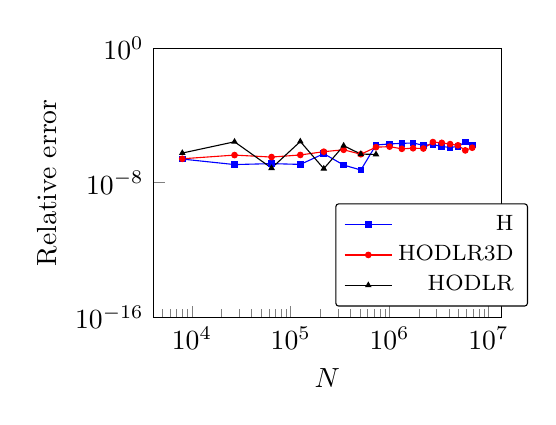
\begin{tikzpicture}[every mark/.append style={mark size=1pt}]
	\begin{axis}[	xlabel={$N$},
	ylabel={Relative error},
%		legend pos=south east,
		legend style={
                at={(0.8,0.04)},
               anchor=south,
               legend columns=1,
               cells={anchor=east},
              font=\footnotesize,
               rounded corners=1pt,
               },
		xmode = log,
	    ymode = log,
	   % xmin = 1e3,
	   % xmax = 1e6,
	    ymin = 1e-16,
	    ymax = 1e-0,
	   % xtick={1e-10, 1e-8, 1e-6,  1e-4,  1e-2},
	   % ytick={1e-8, 1e-6,  1e-4,  1e-2, 1e-0}
		]
		
		\addplot[
		color=blue,
		mark=square*,
		] coordinates {
(8000,2.557150e-07)
(27000,1.202710e-07)
(64000,1.370560e-07)
(125000,1.230890e-07)
(216000,5.331510e-07)
(343000,1.123290e-07)
(512000,5.729630e-08)
(729000,1.751730e-06)
(1000000,2.027060e-06)
(1331000,2.202360e-06)
(1728000,2.307030e-06)
(2197000,1.690290e-06)
(2744000,1.829160e-06)
(3375000,1.463420e-06)
(4096000,1.213900e-06)
(4913000,1.479610e-06)
(5832000,2.596010e-06)
(6859000,1.748060e-06)
		};
		\addplot[
		color=red,
		mark=*,
		] coordinates {
(8000,2.657270e-07)
(27000,4.404200e-07)
(64000,3.362950e-07)
(125000,4.484270e-07)
(216000,7.017800e-07)
(343000,9.128360e-07)
(512000,4.942570e-07)
(729000,1.300020e-06)
(1000000,1.400770e-06)
(1331000,1.041650e-06)
(1728000,1.125510e-06)
(2197000,1.085220e-06)
(2744000,2.611650e-06)
(3375000,2.357380e-06)
(4096000,1.979970e-06)
(4913000,1.679470e-06)
(5832000,8.381420e-07)
(6859000,1.209460e-06)
% (7077888,2.033970e-06)
		};
\addplot[
		color=black,
		mark=triangle*,
		] coordinates {
(8000,5.823700e-07)
(27000,2.719750e-06)
(64000,7.445260e-08)
(125000,2.823590e-06)
(216000,6.860880e-08)
(343000,1.586930e-06)
(512000,5.050740e-07)
(729000,4.830780e-07)
		};
		\legend{H, HODLR3D, HODLR}
		\end{axis}
\end{tikzpicture}
\end{document}